\section{Full sensitivity of the ledger}\label{sec:app-sensitivity}

Table~\ref{tab:sensitivity} gives the recall and the miss composition under every read-out, tiling, operating point and detector referenced in Section~\ref{sec:res-robust}, and Fig.~\ref{fig:sensitivity} plots recall against the output cap together with the composition of small-object misses. Across the whole sweep the tail-small no-candidate count stays between 13 and 20 of 38, while the head-small pre-suppression mass moves sharply with the merge rule, which is the quantitative basis for the claim that the tail-small bottleneck is configuration-independent whereas the head-small profile is not.

\begin{table}[!htbp]
\fontsize{6pt}{7pt}\selectfont
\caption{Sensitivity of recall and of the recovery-ceiling partition to the read-out, tiling, operating point and detector (audit set).}
\label{tab:sensitivity}
\begin{tabular*}{\textwidth}{@{\extracolsep{\fill}}p{3.6cm}rrrrrr}
\toprule
Configuration & R all & P all & R small & \shortstack{Tail-small\\det.} & \shortstack{Small misses\\N/P/H (\%)} & \shortstack{Tail-small\\misses N/P/H} \\
\midrule
\multicolumn{7}{l}{\textit{Primary}} \\
YOLO11n, $T$=320/0.25, GREEDYNMM-IOS, $\tau$=0.25, cap 100 & 79.3 & 48.9 & 75.2 & 11/38 & 15/36/48 & 16/2/9 \\
\multicolumn{7}{l}{\textit{Read-out}} \\
NMS-IoU 0.5 (class-aware) & 82.9 & 46.1 & 81.8 & 10/38 & 21/6/73 & 16/2/10 \\
GREEDYNMM-IOS, class-agnostic & 74.1 & 50.9 & 70.9 & 10/38 & 13/59/28 & 16/6/6 \\
Threshold before merge (SAHI deployment order) & 82.6 & 50.9 & 80.8 & 11/38 & 20/79/1 & 16/11/0 \\
Full image only (no slicing) & 73.5 & 67.1 & 68.4 & 5/38 & 28/17/55 & 20/1/12 \\
\multicolumn{7}{l}{\textit{Tiling}} \\
$T$=256, overlap 0.25 & 76.0 & 43.2 & 71.9 & 11/38 & 14/31/55 & 13/2/12 \\
$T$=480, overlap 0.25 & 78.9 & 51.7 & 73.9 & 12/38 & 14/51/35 & 15/5/6 \\
$T$=320, overlap 0 (positive control) & 79.3 & 51.1 & 75.6 & 11/38 & 17/33/51 & 18/1/8 \\
\multicolumn{7}{l}{\textit{Operating point}} \\
$\tau$=0.10 & 84.3 & 33.5 & 81.2 & 16/38 & 20/48/32 & 16/2/4 \\
$\tau$=0.40 & 72.8 & 60.0 & 67.3 & 6/38 & 12/28/61 & 16/2/14 \\
Global cap 20 & 61.8 & 54.7 & 53.0 & 10/38 & 8/19/73 & 16/2/10 \\
Global cap 300 & 79.4 & 48.8 & 75.3 & 11/38 & 15/37/48 & 16/2/9 \\
Per-class cap 5 & 47.8 & 48.5 & 38.7 & 11/38 & 6/15/79 & 16/2/9 \\
Per-class cap 20 & 71.6 & 50.0 & 66.3 & 11/38 & 11/27/62 & 16/2/9 \\
\multicolumn{7}{l}{\textit{Detector}} \\
FCOS-R50-FPN, primary pipeline & 48.9 & 6.5 & 51.4 & 4/38 & 12/76/12 & 9/18/7 \\
FCOS-R50-FPN, NMS-IoU 0.5 & 89.9 & 11.2 & 85.3 & 15/38 & 40/7/53 & 10/4/9 \\
FCOS-R50-FPN, threshold before merge & 85.7 & 11.4 & 79.9 & 19/38 & 29/47/24 & 10/7/2 \\
\bottomrule
\end{tabular*}
\footnotetext{N/P/H: no candidate / pre-suppression only / post-hoc recoverable. R, P in \%. Tail-small det.: detected/total.}
\end{table}


\begin{figure}[!htbp]
    \centering
    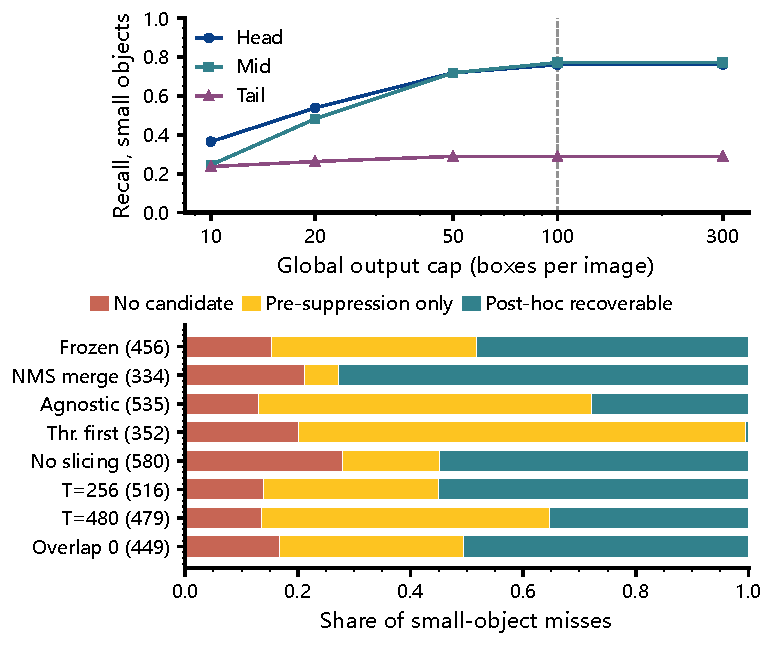
\includegraphics[width=0.98\textwidth,height=0.8\textheight,keepaspectratio]{../figures/fig_sensitivity.pdf}
    \caption{Sensitivity of the ledger. Top: recall of small objects per stratum against the global output cap (frozen cap 100 dashed). Bottom: composition of small-object misses under the frozen pipeline and alternative read-outs and tilings (number of misses in brackets).}
    \label{fig:sensitivity}
\end{figure}

\section{The second detector in full}\label{sec:app-fcos}

The partition under FCOS-ResNet50-FPN, referenced in Section~\ref{sec:res-detector}, is given in Table~\ref{tab:partition-fcos}: because the undertrained detector floods each tile with low-score boxes, the merge stage dominates every stratum, and the no-candidate column is correspondingly small. Reading past that merge artefact, FCOS leaves 9 of 38 tail-small objects with no candidate, fewer than YOLO11n, which is why the cross-detector message is that candidate formation is detector-dependent.

\begin{table}[!htbp]
\footnotesize
\caption{Recovery-ceiling partition of missed objects (FCOS).}
\label{tab:partition-fcos}
\begin{tabular}{lrrrrrr}
\toprule
Stratum, size & $N$ (groups) & Recall (\%) & Misses & No cand. & Pre-supp. & Post-hoc \\
\midrule
Tail $<32^2$ (primary) & 38 (27) & 10.5 & 34 & 9 (26) & 18 (53) & 7 (21) \\
\quad 95\% CI & & [2, 21] & & [7, 47] & [32, 76] & [10, 34] \\
\quad Tail $<16^2$ & 11 (5) & 18.2 & 9 & 6 & 3 & 0 \\
\quad Tail $16^2$--$32^2$ & 27 (24) & 7.4 & 25 & 3 (12) & 15 (60) & 7 (28) \\
Mid $<32^2$ & 114 (29) & 45.6 & 62 & 5 (8) & 51 (82) & 6 (10) \\
Head $<32^2$ & 1686 (257) & 52.7 & 797 & 92 (12) & 610 (77) & 95 (12) \\
\quad 95\% CI & & [48, 57] & & [9, 14] & [71, 82] & [8, 16] \\
Tail $\geq 32^2$ & 210 (156) & 37.1 & 132 & 9 (7) & 112 (85) & 11 (8) \\
Mid $\geq 32^2$ & 554 (251) & 37.5 & 346 & 15 (4) & 302 (87) & 29 (8) \\
Head $\geq 32^2$ & 1827 (332) & 51.2 & 892 & 23 (3) & 842 (94) & 27 (3) \\
All objects & 4429 (508) & 48.9 & 2263 & 153 (7) & 1935 (86) & 175 (8) \\
\bottomrule
\end{tabular}
\footnotetext{Group-disjoint audit set, frozen FCOS + SAHI ($T$=320, overlap 0.25, GREEDYNMM/IOS 0.5 at the 0.01 floor), operating point score $\geq$0.25 and 100 boxes per image. Miss columns: count (\% of misses); CI rows: 95\% cluster-bootstrap CI over audit groups; rates and CIs are omitted when a cell has $<$10 events or $<$5 groups. Size-matched contrast (tail-small vs head-small standardized to the tail size mix): no-candidate share difference 11.1 pp [-3.8, 26.7], Holm $p$=0.006; pre-suppression-only 1.1 pp [-22.3, 24.9], Holm $p$=0.996; post-hoc-recoverable 13.6 pp [1.4, 27.6], Holm $p$=0.013.}
\end{table}


The same contrast is visible in the stacked partition and in the stage-survival profile for FCOS (Figs.~\ref{fig:partition-fcos} and~\ref{fig:stage-survival-fcos}), which mirror the YOLO11n figures in the main text and let the two detectors be compared panel by panel.

\begin{figure}[!htbp]
    \centering
    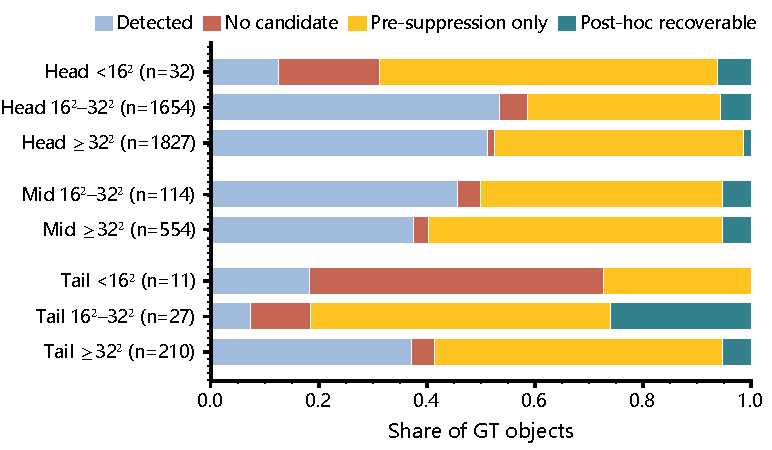
\includegraphics[width=0.98\textwidth,height=0.8\textheight,keepaspectratio]{../figures/fig_partition_fcos.pdf}
    \caption{Recovery-ceiling partition of every audit object under the second detector (FCOS-ResNet50-FPN, SAHI $T$=320, overlap 0.25, frozen GREEDYNMM-IOS merge). Categories and layout match Fig.~\ref{fig:partition}.}
    \label{fig:partition-fcos}
\end{figure}

\begin{figure}[!htbp]
    \centering
    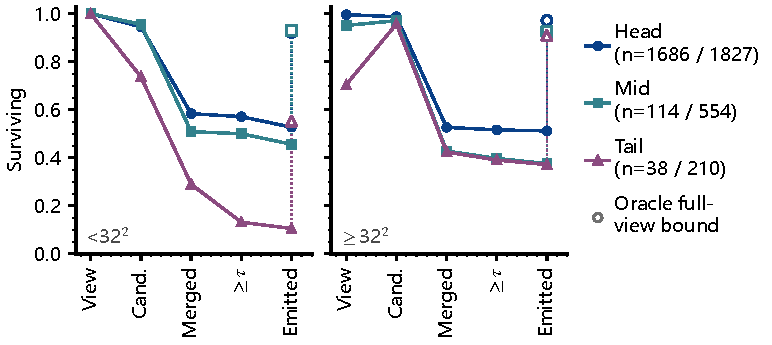
\includegraphics[width=0.98\textwidth,height=0.8\textheight,keepaspectratio]{../figures/fig_stage_survival_fcos.pdf}
    \caption{Stage-survival profile of the per-object ledger on the audit set under FCOS-ResNet50-FPN (SAHI $T$=320, overlap 0.25). Axes match Fig.~\ref{fig:stage-survival}: left, objects smaller than $32^2$; right, larger objects; hollow markers are the oracle full-view read-out.}
    \label{fig:stage-survival-fcos}
\end{figure}

The same-dump post-processing methods behave consistently on FCOS as well (Table~\ref{tab:methods-fcos}): rescoring and calibration recover only post-hoc-recoverable misses, and against an NMS-based comparator the class-conditional read-out is again NO-GO, so the pre-registered negative increment on the primary detector is not reversed by the second.

\begin{table}[!htbp]
\fontsize{6pt}{7pt}\selectfont
\caption{Same-dump post-processing methods on the audit set (FCOS; parameters fit by 5-fold group cross-fitting).}
\label{tab:methods-fcos}
\begin{tabular*}{\textwidth}{@{\extracolsep{\fill}}p{3cm}rrrrrrrrr}
\toprule
Method & \multicolumn{4}{c}{Own operating point} & \multicolumn{5}{c}{Matched false positives} \\ \cmidrule(lr){2-5}\cmidrule(lr){6-10} & R all & \shortstack{Tail\\small} & \shortstack{P\\head} & FP & R all & \shortstack{R head\\small} & \shortstack{Tail\\small} & \shortstack{Recov.\\P/H/N} & Lost \\
\midrule
SAHI baseline (frozen) & 48.9 & 4/38 & 11.6 & 31226 & 48.9 & 52.7 & 4/38 & 0/0/0 & 0 \\
NorCal-style prior correction & 42.9 & 7/38 & 18.8 & 33743 & 42.8 & 41.9 & 7/38 & 0/10/0 & 279 \\
Class$\times$size thresholds & 24.4 & 2/38 & 5.2 & 32691 & 19.4 & 21.5 & 1/38 & 0/2/0 & 1310 \\
Na-style rescoring, class-agnostic & 47.4 & 4/38 & 14.8 & 24582 & 48.0 & 51.4 & 5/38 & 0/49/0 & 89 \\
Na-style rescoring, per class & 41.0 & 4/38 & 17.9 & 16355 & 44.7 & 47.4 & 5/38 & 0/42/0 & 227 \\
Multi-label evidence + SAHI merge + thr. & 24.4 & 2/38 & 5.2 & 32691 & 19.4 & 21.5 & 1/38 & 0/2/0 & 1310 \\
Peak read-out on std evidence + thr. & 69.5 & 6/38 & 60.2 & 2897 & 88.9 & 85.8 & 20/38 & 1812/20/2 & 62 \\
CCPR without class$\times$size thr. & 90.0 & 18/38 & 19.2 & 32200 & 89.9 & 86.1 & 18/38 & 1829/10/2 & 27 \\
CCPR (multi-label peak read-out + thr.) & 69.5 & 6/38 & 60.2 & 2897 & 88.9 & 85.8 & 20/38 & 1812/20/2 & 62 \\
\bottomrule
\end{tabular*}
\footnotetext{R: recall@0.5 (\%); P head: precision of emitted head-class boxes (\%); tail-small: detected/total. Matched FP: one global threshold per method chosen so that its total false positives do not exceed the baseline's. Recov.\ P/H/N: baseline misses recovered at matched FP, by the baseline's recovery-ceiling category (pre-suppression only / post-hoc recoverable / no candidate); Lost: baseline detections no longer detected.}
\end{table}


\section{Training records}\label{sec:app-training}

For reproducibility, Fig.~\ref{fig:training} shows the training-loss curves of the two frozen RicePest-30 detectors; no validation data were used for checkpoint selection, so the audit set never influenced the weights that produced the results above.

\begin{figure}[!htbp]
    \centering
    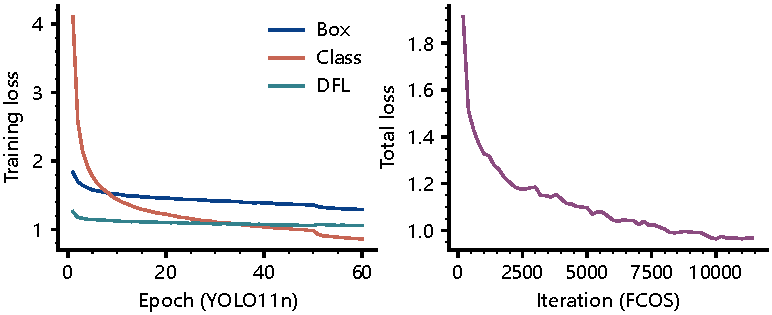
\includegraphics[width=0.98\textwidth,height=0.8\textheight,keepaspectratio]{../figures/fig_training.pdf}
    \caption{Training losses of the two frozen RicePest-30 detectors (no validation data were used for checkpoint selection).}
    \label{fig:training}
\end{figure}
